\documentclass{article}

\usepackage{amsmath,amssymb,scalerel,amsthm}
\usepackage{derivative}
\usepackage{mathtools}
\usepackage{color}
\usepackage{tikz}

\title{Geometry I}
\author{Alessio Esposito}

\newtheorem{theorem}{Theorem}
\newtheorem{proposition}{Proposition}
\newtheorem{definition}{Definition}
\newtheorem{corollary}{Corollary}
\newtheorem{observation}{Obs}

\begin{document}
% List of formulas for two lines $r$ and $r_1$ passing rispectively through the points $Q\equiv(a,b,c)$ and $Q_1\equiv(a_1,b_1,c_1)$. This list covers also other formulas with the following objects:
% \begin{itemize}
%     \item a point $P_0\equiv(x_0,y_0,z_0)$
% \end{itemize} 
    \subsection*{Distance between lines}
        \begin{flalign*}
            d(r,r_1)=\frac{\begin{vmatrix}a - a_1 & b -b_1 & c - c_1 \\ l & m & n \\ l_1 & m_1 & n_1\end{vmatrix}}{\sqrt{\begin{vmatrix}m & n \\ m_1 & n_1\end{vmatrix}^2 + \begin{vmatrix}l & n \\ l_1 & n_1\end{vmatrix}^2 + \begin{vmatrix}l & m \\ l_1 & m_1\end{vmatrix}^2} } \ Q\equiv(a,b,c) \ Q_1\equiv(a_1,b_1,c_1)
        \end{flalign*}
        Where $r = <\vec{a}(l,m,n)>$ and $r_1 = <\vec{a_1}(l_1,m_1,n_1)>$ passing through $Q$ and $Q_1$
    \subsection*{Common perpendicular between two lines}
        \begin{gather*}
            \begin{vmatrix}
                X - a & Y - b & Z - c \\
                \beta_1 & \beta_2 & \beta_3 \\
                l & m & n
            \end{vmatrix} = 0 \\
            \begin{vmatrix}
                X - a_1 & Y - b_1 & Z - c_1 \\
                \beta_1 & \beta_2 & \beta_3 \\
                l_1 & m_1 & n_1
            \end{vmatrix} = 0
        \end{gather*}
        Where $<\beta_1,\beta_2,\beta_3> = <\vec{a}\times\vec{a_1}>$ \\
    % Given a plane $\pi$, a point $P_0\equiv(x_0,y_0,z_0)$ and a line $r$ one has the following:
    \subsection*{Distance between a plane and a point}
        \begin{flalign*}
            d(P_0,\pi)=\frac{|Ax_0 + By_0+ Cz_0 + D|}{\sqrt{A^2 + B^2 + C^2}}_{P_0\equiv(x_0,y_0,z_0)}
        \end{flalign*}
    \subsection*{Distance between a point and a line}
        \begin{flalign*}
            d(P_0,r) = \frac{\begin{vmatrix}y_0 - b & z_0 - c \\ m & n \end{vmatrix}^2 + \begin{vmatrix}x_0 - a & z_0 - c \\ l & n\end{vmatrix}^2 + \begin{vmatrix}x_0 - a & y_0 - b \\ l & m\end{vmatrix}^2}{\sqrt{l^2 + m^2 + n^2}}_{\ P_0\equiv(x_0,y_0,z_0)}
        \end{flalign*}
    \subsection*{Angle between two planes}
        \begin{flalign*}
            \cos\varphi = \frac{<n,n_1>}{\left\lVert n \right\rVert \left\lVert n_1 \right\rVert} = \frac{AA_1 + BB_1 + CC_1}{\sqrt{A^2 + B^2 + C^2}\sqrt{A_1^2 + B_1^2 + C_1^2}}     
        \end{flalign*}  
    \subsection*{Angle between a line and a plane} 
        \begin{flalign*}
            \sin\varphi = \frac{Al + Bm + Cn}{\sqrt{A^2 + B^2 + C^2}\sqrt{l^2 + m^2 + n^2}}     
        \end{flalign*}
        \newpage
    \subsection*{Plane passing for three points}
        \begin{flalign*}
            \pi = \begin{vmatrix}
                X - x_0 & Y - y_0 & Z - z_0 \\ x_1 - x_0 & y_1 - y_0 & z_1 - z_0 \\ x_2 - x_0 & y_2 - y_0 & z_2 - z_0
            \end{vmatrix}=0_{\ P_0 \equiv (x_0,y_0,z_0),P_1 \equiv (x_1,y_1,z_1), P_2 \equiv (x_2,y_2,z_2)} 
        \end{flalign*}
        
    \subsection*{Parametric equations of a plane}
        \begin{gather*}
            x = q_1 + a_1u + b_1v \\
            y = q_2 + a_2u + b_2v \\
            z = q_3 + a_3u + b_3v
        \end{gather*}
        Where $\left\{ \vec{a}(a_1,a_2,a_3), \vec{b}(b_1,b_2,b_3)  \right\}$ is the basis and $Q\equiv(q_1,q_2,q_3)$ is a point      
        
    \subsection*{Cartesian equation of a plane}
        \begin{flalign*}
            \begin{vmatrix}
                X - q_1 & Y-q_2 & Z-q_3 \\
                a_1 & a_2 & a_3 \\
                b_1 & b_2 & b_3
            \end{vmatrix} = 0
        \end{flalign*}
        With $A = \begin{vmatrix} a_2 & a_3 \\ b_2 & b_3 \end{vmatrix}$, $B = -\begin{vmatrix} a_1 & a_3 \\ b_1 & b_3 \end{vmatrix}$, $C = \begin{vmatrix} a_1 & a_2 \\ b_1 & b_2 \end{vmatrix}$ one has the following:
        \begin{equation*}
            A\left( X - q_1 \right) + B\left( Y - q_2 \right) + C\left( Z - q_3 \right) = 0
        \end{equation*}
    \subsection*{Directional vector of a line}
        \begin{gather*}
            r =\begin{cases}
                AX + BY + CZ + D = 0 \\
                A'X + B'Y + C'Z + D' = 0
            \end{cases} \\
            l = \begin{vmatrix}
                B & C \\ B' & C'
            \end{vmatrix}, \
            m = - \begin{vmatrix}
                A & C \\ A' & C'
            \end{vmatrix}, \
            n = \begin{vmatrix}
                A & B \\ A' & B'
            \end{vmatrix}    
        \end{gather*}
    \subsection*{Cartesian equations of a line}
        \begin{flalign*}
            \left(\begin{matrix}
                X-a & Y-b &Z-c \\
                l & m & n
            \end{matrix}\right)_{Q\equiv (a,b,c), \vec{v}(l,m,n)}
        \end{flalign*}
        The equatons are the minors of the above matrix equal to zero:
        \begin{gather*}
            m\left( X - a \right) - l\left( Y - b\right) = 0 \\
            n\left( X - a \right) - l\left( Z - c\right) = 0  
        \end{gather*}
    
    \newpage
    \subsection*{Vectorial product}
        let $\left\{ \vec{i},\vec{j},\vec{k} \right\}$ be an orthonormal basis of $\mathbb{R}^3$ then we have the following: 
        \begin{gather*}
            \vec{i} \times \vec{j} = -\vec{j} \times \vec{i} = \vec{k} \\
            \vec{j} \times \vec{k} = -\vec{k} \times \vec{j} = \vec{i} \\
            \vec{k} \times \vec{i} = -\vec{i} \times \vec{k} = \vec{j} \\
            \vec{i} \times \vec{i} = \vec{j} \times \vec{j} = \vec{k} \times \vec{k} = \vec{0} 
        \end{gather*}
        The \textbf{v.p.} between two arbitrary vectors $\vec{v}(v_1,v_2,v_3)$ and $\vec{w}(w_1,w_2,w_3)$ of $\mathbb{R}^3$ is:
        \begin{equation*}
            \vec{v} \times \vec{w} = \left(v_2w_3 - v_3w_2\right)\vec{i} + \left(v_3w_1 - v_1w_3\right) \vec{j} + \left(v_1w_2 - v_2w_1\right) \vec{k} \ \ \triangle 
        \end{equation*}
        That can be seen as:
        \begin{equation*}
            \vec{v} \times \vec{w} = \begin{vmatrix}
                \vec{i} && \vec{j} && \vec{k} \\
                v_1 && v_2 && v_3 \\
                w_1 && w_2 && w_3
            \end{vmatrix}
        \end{equation*}
        By theory the $\triangle$ is defined by the minors of second order taken with the criteria $+,-,+$ of the matrix:
        \begin{gather*}
            \left(\begin{matrix}
                v_1 && v_2 && v_3 \\
                w_1 && w_2 && w_3
            \end{matrix}\right) 
        \end{gather*}
        One can remind easily the propreties of $\vec{i},\vec{j},\vec{k}$ with the scheme:
        \begin{center}
            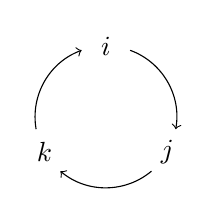
\begin{tikzpicture}[->,scale=.9]
                \node (i) at (90:1cm)  {$i$};
                \node (j) at (-30:1cm) {$j$};
                \node (k) at (210:1cm) {$k$};
             
                \draw (70:1cm)  arc (70:-10:1cm);
                \draw (-50:1cm) arc (-50:-130:1cm);
                \draw (190:1cm) arc (190:110:1cm);
             \end{tikzpicture}
        \end{center}
        \subsection*{More propreties about the v.p.}
        Let be $\mathfrak{v},\mathfrak{w},\mathfrak{u} \in \mathbb{R}^3$ and $c\in \mathbb{R}$ then one has
        \begin{gather*}
            \mathfrak{v} \times \mathfrak{w} = -\mathfrak{w} \times \mathfrak{v} \\
            \mathfrak{v} \times \left( \mathfrak{w} + \mathfrak{u}\right) = \mathfrak{v} \times \mathfrak{w} + \mathfrak{v} \times \mathfrak{u} \\
            c\left(\mathfrak{v}\times \mathfrak{w}\right) = \left( c\mathfrak{v}\right) \times \mathfrak{w} = \mathfrak{v} \times \left(c\mathfrak{w}\right) \\
        \end{gather*}


\end{document}